\section{Implementación del SGDW}\label{sec:sgdw}  % MARK: SGDW

\RED[inline]{Revisar este párrafo reu 02/07}

En esta sección se presenta la implementación del SGDW. Se empieza explicando cómo se interpreta una imagen como una medida. Luego, se presentan las ligeras modificaciones al algoritmo original para que se pueda trabajar con medidas discretas. Posteriormente, se presentan los experimentos realizados con distintas medidas, y se discuten los resultados obtenidos.

\subsection{Interpretación de una Imagen como Medida}\label{ssec:interpr-imagen-medida}  % MARK: - Interpretación de una Imagen como Medida

Recordar que si $\mu\in \ProbSpace[\cX] $ es una medida discreta, entonces esta queda definida de la siguiente forma:
\begin{equation}\label{eq:medida-discreta}
    \mu = \sum_{i=1}^{n} m_i \delta_{x_i},
\end{equation}
donde $m \in \Simplex[n]$ es un vector de probabilidad en el Simplex y $ \left\{ x_1, \dots, x_n \right\} \subseteq \cX $ son sus posiciones.

En el caso de una imagen, esta se puede interpretar como una medida discreta, si se define $\cX \eqdef \left\{ x_1, \dots, x_n \right\} \subseteq \R^2$ como las posiciones de los píxeles, con $n \eqdef n_1 \times n_2$; y $m \in \Simplex[n]$ como el vector de probabilidad representando las intensidades de los píxeles. En este caso, si se asume que el espacio de imágenes es el espacio de probabilidad $\ProbSpace[\cX] $, entonces las distribuciones que muestrean imágenes corresponderían a distribuciones en el espacio $\ProbSpace[\ProbSpace[\cX] ] $.

\RED[inline]{Revisar este párrafo reu 02/07}
Las distribuciones que provienen de una imagen se implementan de manera eficiente tanto en tiempo y en memoria, utilizando su matriz de escala de grises. En la Figura~\ref{fig:face-example} se muestra un ejemplo de una distribución que proviene de una imagen, donde se presenta la imagen y su histograma para $n=1000$ muestras.

\begin{figure}[htbp]
    \centering
    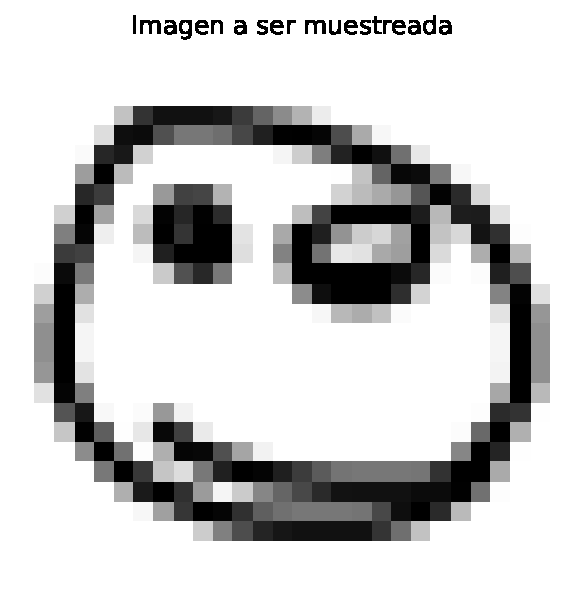
\includegraphics[height=6cm]{img/distr_draw/face_distrib.pdf}
    \hspace{2cm}
    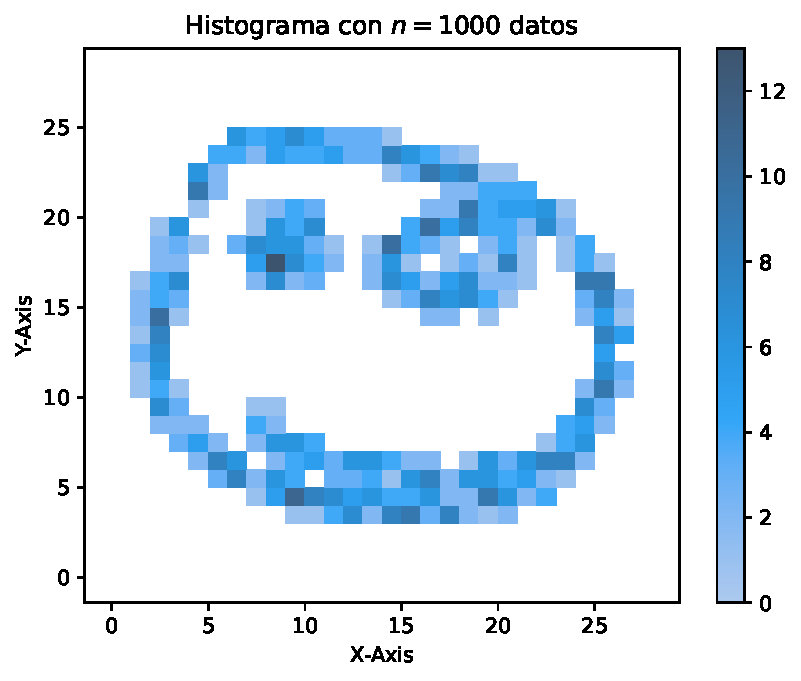
\includegraphics[height=6cm]{img/distr_draw/face_hist.pdf}
    \caption{A la izquierda, una imagen del dibujo de una cara. A la derecha, un histograma de $n=1000$ muestras obtenidas a partir de esta imagen.}
    \label{fig:face-example}
\end{figure}

\subsection{Implementación del Algoritmo}\label{ssec:implementacion-algoritmo}  % MARK: - Implementación del Algoritmo

Dado que el Algoritmo~\ref{alg:sgdw-clasico} está diseñado para medidas absolutamente continuas, se reinterpreta este algoritmo para que se pueda trabajar con medidas discretas. Para ello, se destaca que la Definición~\ref{def:sgdw} se puede reinterpretar como la $\eta_k$-interpolación geodésica entre las medidas $\mu_k$ y $\tilde \mu_k$, mientras que la Definición~\ref{def:bsgdw} se puede reinterpretar como el baricentro de las medidas $\qty( \mu_k, \tilde\mu_k^{(1)}, \dots, \tilde\mu_k^{(S_k)} )$ con pesos $\qty(1-\eta_k, \frac{\eta_k}{S_k}, \dots, \frac{\eta_k}{S_k}) \in \Simplex[S_k+1]$. De este modo, el Algoritmo~\ref{alg:sgdw-clasico} se extiende de la siguiente manera:
\begin{algorithm}[H]
    \caption{SGDW General}
    \label{alg:sgdw-general}
    \begin{algorithmic}[1]
        \Require Acceso a las muestras de $\Gamma(\dd \mu) \in \ProbSpace[\ProbSpace]$, un esquema de paso $(\eta_k)_k \in [0, 1]^\N$ y un esquema de paso $(S_k)_k \in \N^\N$.
        \State{$k\gets0$}
        \State{Muestrear $\mu_0 \sim \Gamma$}
        \Repeat
        \State{Muestrear $\tilde \mu_k^{(1)}, \dots, \tilde \mu_k^{(S_k)} \simiid \Gamma$}
        \State{$\gamma\gets\qty(1-\eta_k, \frac{\eta_k}{S_k}, \dots, \frac{\eta_k}{S_k})$}
        \State Definir $\mu_k$ como el baricentro de $\qty( \mu_k, \tilde\mu_k^{(1)}, \dots, \tilde\mu_k^{(S_k)} )$ con pesos $\gamma$.
        \State{$k\gets k+1$}
        \Until{un criterio de detención ha sido alcanzado.}
        \State\Return $\mu_k$
    \end{algorithmic}
\end{algorithm}

\RED[inline]{Revisar este párrafo reu 02/07}
Se destaca que en el Algoritmo~\ref{alg:sgdw-general} se mantiene la versión de la secuencia por lotes. Esto es debido para mantener una mayor generalidad, pues el caso original del Algoritmo~\ref{alg:sgdw-clasico} se recupera considerando $S_k=1,\ \forall k\in\N$.

\RED[inline]{Hay que revisar esta sección para ver cómo se pueden combinar o modificar.}

Como se está trabajando con imágenes, se puede aprovechar su estructura para calcular una estimación de los baricentros de manera más eficiente, utilizando el algoritmo de Baricentros de Wasserstein Convolucionales \cite{solomon2015convolutional} o su versión Insesgada (\textit{Debiased} en inglés) \cite{janati2020debiased}. Sin embargo, el Algoritmo~\ref{alg:sgdw-general} es lo suficientemente general para ser aplicado a cualquier medida discreta, utilizando por ejemplo, la estimación del algoritmo de Sinkhorn \cite{cuturi2013sinkhorn}.

Todos estos métodos de cálculo de baricentros se implementan de manera eficiente utilizando la librería de \textit{Python Optimal Transport} (POT) \cite{flamary2021pot}, donde además esta librería admite la paralelización de los cálculos por medio de la computación de Propósito General en Unidades de Procesamiento Gráfico (GPGPU por sus siglas en inglés) \cite{owens2008gpu}. En la implementación, se mantienen las versiones tanto para imágenes como para medidas discretas genéricas, para mayor generalidad y versatilidad.

\subsection{Experimentos con distintas medidas}\label{ssec:muestreando-gamma}  % MARK: - Muestreando de la Medida Gamma


Se considera una medida de referencia $\Prob_X \in \ProbSpace[\ProbSpace[\cX]]$ que corresponde a la forma ideal\FM{Con esto me esto refiriendo que no se utiliza directamente el data set, si no más bien una versión teórica y continua del mismo, donde nosotros tenemos acceso a esa variedad a través de muestras, y que la utilizamos como una aproximación de dicha variedad.} del conjunto de datos \textit{Quick, Draw!} \cite{jongejan2016quick}. Se desea calcular el baricentro de esta medida, utilizando el Algoritmo~\ref{alg:sgdw-general}. Para ello, se obtendrán dos aproximaciones. La primera, es la empírica:
\begin{equation}
    \hat \Prob_X = \frac{1}{N} \sum_{i=1}^{N} \delta_{\mu_i},
\end{equation}
donde $\left\{ \mu_i \right\}_{i=1}^{N} \subseteq \ProbSpace[\cX] $ es el conjunto de datos obtenido de la Sección~\ref{ssec:preparacion-dataset}, y $N$ es el tamaño del conjunto de datos. La segunda, es la medida generada por la WGAN $G_\theta : \cZ \to \ProbSpace[\cX]$, entrenada como se explica en el Capítulo~\ref{chap:WAE-WGAN}:
\begin{equation}
    \tilde \Prob_X
    = \pf{G_\theta} \Prob_Z
    %\int_{\cZ} \delta_{G_\theta(z)} (\dd \mu) \; \Prob_Z(\dd z),
\end{equation}
donde $\Prob_Z$ es la medida del espacio latente (en este caso, una distribución normal estándar).

Como ambas son estimaciones de la medida de referencia $\Prob_X$, se espera que el baricentro de estas medidas sean similares entre sí.

\subsection{Resultados y Discusión}\label{ssec:sgdw-resultados-discusion}  % MARK: -- Resultados y Discusión

\FM[inline]{En esta sección se podría incluir el cálculo de un baricentro, tanto del dataset como de la GAN}

\subsection{Conclusiones}\label{ssec:sgdw-conclusiones}  % MARK: -- Conclusiones

\FM[inline]{Insertar aquí alguna conclusión}

\FM[inline]{Una conclusión que se me ocurre es como los dos baricentros, el del conjunto de datos y el de la GAN se parecen, algo que debería de pasar puesto que ambos están aproximando a alguna medida de referencia $\Prob_X$}

